% Chapter Template

\chapter{Ensayos y resultados} % Main chapter title

\label{Chapter4} % Change X to a consecutive number; for referencing this chapter elsewhere, use \ref{ChapterX}

%----------------------------------------------------------------------------------------
%	SECTION 1
%----------------------------------------------------------------------------------------
En este capítulo se describen los ensayos realizados y se presentan y comparan los resultados obtenidos.

\section{Banco de pruebas}
\label{sec:pruebasHW}

Para el desarrollo del presente proyecto se utilizaron 3 bancos de pruebas, con las siguientes especificaciones técnicas:

\begin{itemize}
\item Banco de pruebas Laptop MacBook Pro - hardware disponible:
	\begin{itemize}
	\item OS: MacOS Sonoma 14.
	\item CPU: Apple M1 Pro.
	\item RAM: 32 GB.
	\item GPU: No contiene.
	\end{itemize}
\item Banco de pruebas Laptop ASUS TUF GAMING F15 - hardware disponible:
	\begin{itemize}
	\item OS: Windows 11.
	\item CPU: Intel(R) Core(TM) i5-11260H.
	\item RAM: 16 GB.
	\item GPU: NVIDIA GeForce RTX 3050.
	\end{itemize}
\item Banco de pruebas Google Colab Pro - hardware disponible:
	\begin{itemize}
	\item OS: desconocido.
	\item CPU: desconocido.
	\item RAM: 12,5 GB.
	\item GPU: T4.
	\end{itemize}
\end{itemize}

\section{Desempeño de modelos}
\label{sec:desempeñoMod}

Para medir el desempeño de los modelos de IA utilizados durante la ejecución de este trabajo, se decidió emplear la métrica mAP. Esta métrica evalúa tanto la clasificación del objeto como la ubicación del \textit{bounding box} a través del \textit{Average Precision} (AP) que se representa en la ecuación \ref{eq:AP}.

\begin{equation}
    \label{eq:AP}
    \text{AP} = \frac{1}{n} \sum_{k=1}^n \text{Precisión en } k \times \text{Rel}_{k}
\end{equation}

Donde
\begin{itemize}
    \item \( n \) es el número total de elementos recuperados.
    \item \(\text{Precisión en } k\) es la precisión en el \( k \)-ésimo punto de recuperación.
    \item \(\text{Rel}_{k}\) es un indicador binario que denota si el elemento en el \( k \)-ésimo punto de recuperación es relevante (\( \text{Rel}_{k} = 1 \)) o no relevante (\( \text{Rel}_{k} = 0 \)).
\end{itemize}

Luego, al promediar los valores de AP entre todas las clases, se obtiene respectivamente el mAP y la ecuación queda como se muestra en \ref{eq:mAP}.

\begin{equation}
    \label{eq:mAP}
    \text{mAP} = \frac{1}{C} \sum_{c=1}^C \text{AP}_c
\end{equation}

Donde 
\begin{itemize}
	\item \( C \) es el número total de clases o consultas.
    \item AP es el \textit{Average Precision} calculado para la clase o consulta.
\end{itemize}

\subsection{Desempeño del detector de regla}

Como se mencionó en el capítulo anterior, el detector de la regla tiene como modelo base un YOLOv8n y cumple una función fundamental para la estimación de la longitud de la vareta. Por otro lado, el entrenamiento de este modelo se realizó con los siguientes hiperparámetros:

\begin{itemize}
	\item Épocas: 100.
    \item Tamaño de imagen de entrada: 640 x 640.
    \item \textit{Batch}: 16.
    \item \textit{Learning rate}: 0,01.
\end{itemize}

Los resultados obtenidos para la detección de este elemento contra el conjunto de datos de prueba se observan en la tabla \ref{tab:resultadosRegla}.

\begin{table}[h]
	\centering
	\caption{Métricas de detección para el detector de regla.}
	\begin{tabular}{c c c c c c c}    
		\toprule
		\textbf{Clase}&\textbf{Imágenes}&\textbf{Detecciones}&\textbf{\textit{Precision}} &\textbf{\textit{Recall}}&\textbf{mAP50}&\textbf{mAP50-95}\\
		\midrule
		Regla & 13 & 13 & 0,996 & 1,0 & 0,995 & 0,995\\		
		\bottomrule
		\hline
	\end{tabular}
	\label{tab:resultadosRegla}
\end{table}

Los resultados fueron muy buenos en general. El modelo puede detectar la regla sin dificultad en el 99\% de los casos. Por este motivo, se tomó directamente este modelo para desempeñar la tarea y no se requirió de aumentos de datos o alguna otra técnica de \textit{machine learning}.

\subsection{Desempeño del detector de vareta}

El detector de vareta destinado para el módulo de estimación de longitud, tiene como modelo base un YOLOv8n entrenado bajo los siguientes hiperparámetros:

\begin{itemize}
	\item Épocas: 100.
    \item Tamaño de imagen de entrada: 640 x 640.
    \item \textit{Batch}: 16.
    \item \textit{Learning rate}: 0,01.
\end{itemize}

Para este modelo se hicieron dos pruebas, una sin aumento de datos y otra con aumento. El aumento de datos aplicado corresponde a lo descripto en la sección \ref{aumentoDatos}.

Los resultados obtenidos contra el conjunto de datos de pruebas para el modelo sin aumento de datos se muestran en la tabla \ref{tab:resultadosVareta}.

\begin{table}[h]
	\centering
	\caption{Métricas de detección para el detector de varetas sin aumento de datos.}
	\begin{tabular}{c c c c c c c}    
		\toprule
		\textbf{Clase}&\textbf{Imágenes}&\textbf{Detecciones}&\textbf{\textit{Precision}} &\textbf{\textit{Recall}}&\textbf{mAP50}&\textbf{mAP50-95}\\
		\midrule
		Vareta & 10 & 40 & 1,0 & 0,923 & 0,983 & 0,574\\		
		\bottomrule
		\hline
	\end{tabular}
	\label{tab:resultadosVareta}
\end{table}

Como se puede observar, el modelo sin aumento de datos consigue detectar un total de 40 varetas en 10 imágenes, donde todas las detecciones fueron correctas. Por otro lado, el modelo logra una precisión promedio de detección del 98,3\% cuando se requiere un nivel de confianza igual al 50\%, pero el mAP 50-95, indica que en los casos donde el nivel de confianza esta entre el 50\% y 95\%, la precisión promedio, es de un 57,4\%. Por este motivo, se decidió aplicar aumento de datos.

Los resultados con aumento de datos se pueden observar en la tabla \ref{tab:resultadosVaretaConAug}.

\begin{table}[h]
	\centering
	\caption{Métricas de detección para el detector de varetas con aumento de datos.}
	\begin{tabular}{c c c c c c c}    
		\toprule
		\textbf{Clase}&\textbf{Imágenes}&\textbf{Detecciones}&\textbf{\textit{Precision}} &\textbf{\textit{Recall}}&\textbf{mAP50}&\textbf{mAP50-95}\\
		\midrule
		Vareta & 10 & 40 & 0,974 & 0,975 & 0,976 & 0,702\\		
		\bottomrule
		\hline
	\end{tabular}
	\label{tab:resultadosVaretaConAug}
\end{table}

Luego de aplicar aumento de datos, se observa que el modelo mejoró la cantidad de veces donde detecta de forma precisa a la clase vareta en un 5,2\% con respecto al modelo sin aumento de datos. Por otro lado, también se incrementó la precisión promedio al 70,2\% cuando se tiene un umbral de confianza que va entre 50\% y 95\%.

Con esto se destaca que el aumento de datos mejoró el rendimiento del modelo de forma considerable.

\subsection{Desempeño del detector de estados fenológicos}

La detección de estados fenológicos, como se mencionó en el capítulo anterior, fue probada con dos modelos de IA que se ajustan para este caso de uso. Por un lado, se probó con un detector de dos etapas como es Faster R-CNN y por otro lado con un detector de una etapa como YOLOv8. Ambos casos, se probaron con y sin el uso de aumento de datos. Los resultados fueron los siguientes:

\subsubsection{Faster R-CNN sin aumento de datos}

El entrenamiento del modelo se hizo bajo los siguientes hiperparámentros:

\begin{itemize}
	\item Épocas: 100.
    \item Tamaño de imagen de entrada: 640 x 640.
    \item \textit{Batch}: 4.
    \item \textit{Learning rate}: 0,001.
    \item \textit{Momentum}: 0,9.
    \item \textit{Weight decay}: 0,0005.
    \item \textit{Optimizer}: \textit{Stochastic gradient descent}.
\end{itemize}

Los resultados de detección contra el conjunto de prueba se muestra en la tabla \ref{tab:resultadosFasterSinAug}.

\begin{table}[h]
	\centering
	\caption{Métricas de detección para Faster R-CNN sin aumento de datos.}
	\begin{tabular}{c c c c c c c}    
		\toprule
		\textbf{Clase}&\textbf{Imágenes}&\textbf{mAP}&\textbf{mAP50}&\textbf{mAP> 50}\\
		\midrule
		Todas & 14 & 0,3492 & 0,5970 & 0,3605\\
		Flor abierta & 14 & 0,4313 & - & - \\
		Flor cerrada & 14 & 0,1525 & - & - \\
		Flor sin pétalos & 14 & 0,3735 & - & - \\
		Incierto & 14 & 0,0942 & - & - \\
		Vareta & 14 & 0,6947 & - & - \\		
		\bottomrule
		\hline
	\end{tabular}
	\label{tab:resultadosFasterSinAug}
\end{table}

La precisión promedio de detección entre todas las clases es de un 34,9\%, lo que significa que el modelo tiene una precisión del 34,9\% al detectar las diferentes clases en el conjunto de datos. Además, el modelo logra una precisión de detección del 59,7\% cuando se considera un umbral de confianza igual al 50\% y para detecciones con un nivel de confianza mayor al 50\% se tiene una precisión del 36,1\%.

Por otro lado, al evaluar la precisión promedio de detección por clase, se observa que la categoría vareta es la clase a la que el modelo detecta con mejor precisión promedio con 69,5\%, seguida por flor abierta con 43,13\% y por flor sin pétalos con 37,35\%. Además, se muestra que el modelo detecta con dificultad las categorías flor cerrada con un mAP de 12,25\% e incierto con 9,42\%.

Este bajo porcentaje de mAP para la clase flor cerrada con respecto a las otras categorías presentes, se puede deber al desbalance de datos observado en la sección \ref{desbalanceAfterLabeled} y al rendimiento del modelo al intentar detectar objetos pequeños en la imagen. Adicionalmente, para la categoría incierto no se cuenta con una cantidad de muestras significativas y consistente a través del conjunto de datos, lo que explica la baja precisión promedio obtenida para esta clase.

Para mejorar estos resultados se implementó el aumento de datos mencionado en la sección \ref{aumentoDatos}.

\subsubsection{Faster R-CNN con aumento de datos}

El rendimiento del modelo basado en la métrica mAP, se puede observar en la tabla \ref{tab:resultadosFasterConAug}. 

\begin{table}[h]
	\centering
	\caption{Métricas de detección para Faster R-CNN con aumento de datos.}
	\begin{tabular}{c c c c c c c}    
		\toprule
		\textbf{Clase}&\textbf{Imágenes}&\textbf{mAP}&\textbf{mAP50}&\textbf{mAP> 50}\\
		\midrule
		Todas & 14 & 0,3733 & 0,6328 & 0,3793\\
		Flor abierta & 14 & 0,5143 & - & - \\
		Flor cerrada & 14 & 0,2049 & - & - \\
		Flor sin pétalos & 14 & 0,3290 & - & - \\
		Incierto & 14 & 0,0887 & - & - \\
		Vareta & 14 & 0,7294 & - & - \\		
		\bottomrule
		\hline
	\end{tabular}
	\label{tab:resultadosFasterConAug}
\end{table}

Como se puede observar, se logra mejorar la precisión promedio de detección para las clases flor abierta, flor cerrada y vareta. Con esto, la métrica mAP medida entre todas las clases mejora a 37,33\%, adicionalmente también aumenta a 63,26\% cuando se fija un umbral de confianza de detección igual al 50\% y a un 37,93\% cuando el nivel de confianza en la detección es superior al 50\%.

Se puede concluir que el modelo Faster R-CNN con y sin aumento de datos es bueno para detectar la vareta y las flores en estado abierto. Este comportamiento se puede deber al tamaño de estos objetos en la imagen en comparación con el resto de las categorías que se busca en la detección. Además, la clase flor abierta es la clase más predominante en todas las imágenes según el estudio de los datos realizado en la sección \ref{desbalanceAfterLabeled}, lo que permite que el modelo pueda aprender y reconocer con mayor precisión sus características debido a la abundancia de ejemplos representativos durante el entrenamiento.

\subsubsection{YOLOv8n sin aumento de datos}

Se puede observar en la tabla \ref{tab:resultadosYoloSinAug} el resultado obtenido con YOLOv8n sin aumento de datos, con 14 imágenes del conjunto de pruebas y bajo los siguientes parámetros de entrenamiento:

\begin{itemize}
	\item Épocas: 100.
    \item Tamaño de imagen de entrada: 640 x 640.
    \item \textit{Batch}: 16.
    \item \textit{Learning rate}: 0,01.
\end{itemize}

\begin{table}[h]
	\centering
	\caption{Métricas de detección para YOLOv8n sin aumento de datos.}
	\begin{tabular}{c c c c c c c}    
		\toprule
		\textbf{Clase}&\textbf{Imágenes}&\textbf{mAP50}&\textbf{mAP>50}\\
		\midrule
		Todas & 14 & 0,645 & 0,418\\
		Flor abierta & 14 & 0,905 & 0,611 \\
		Flor cerrada & 14 & 0,614 & 0,251 \\
		Flor sin pétalos & 14 & 0,588 & 0,363 \\
		Incierto & 14 & 0,122 & 0,065 \\
		Vareta & 14 & 0,994 & 0,802 \\		
		\bottomrule
		\hline
	\end{tabular}
	\label{tab:resultadosYoloSinAug}
\end{table}
\newpage
Se puede observar que la precisión promedio de todas las clases obtenida por YOLOv8n es de 64,5\% para el mAP 50. Lo que supera al mAP 50 obtenido con el modelo Faster R-CNN con y sin aumento de datos.

Las clases que este modelo detecta con más precisión, son: vareta, flor abierta y flor cerrada. La diferencia y mejora contra Faster R-CNN se puede observar también al comparar la métrica mAP obtenida para todas las clases donde este modelo se desempeñó mejor. Como ejemplo se tiene la clase vareta, donde se obtuvo un 69,5\% con Faster R-CNN. Esta misma clase que también fue la mejor para el modelo YOLOv8n, tuvo un 99,4\% que representa una mejora del 29,9\%.

Por otro lado, ambos modelos  logran detectar con alta precisión la clase vareta y esto se puede deber al tamaño de este objeto en la imagen. Además, es seguida por la clase flor abierta que, como se mencionó anteriormente, contiene una cantidad de muestras representativas que ayudan al modelo a reconocer los patrones de esta clase. Por último, se destaca la categoría incierto, que tanto este modelo como Faster R-CNN no logran reconocer durante la detección en su totalidad.

La matriz de confusión normalizada mostrada en la figura \ref{fig:cfmatriznorm}, indica que muchas de las veces que se tiene la clase incierto, el modelo la predice como flor abierta. Esto demuestra que el modelo no logró aprender correctamente los patrones que identifican dicha clase durante el entrenamiento.

\begin{figure}[ht]
	\centering
	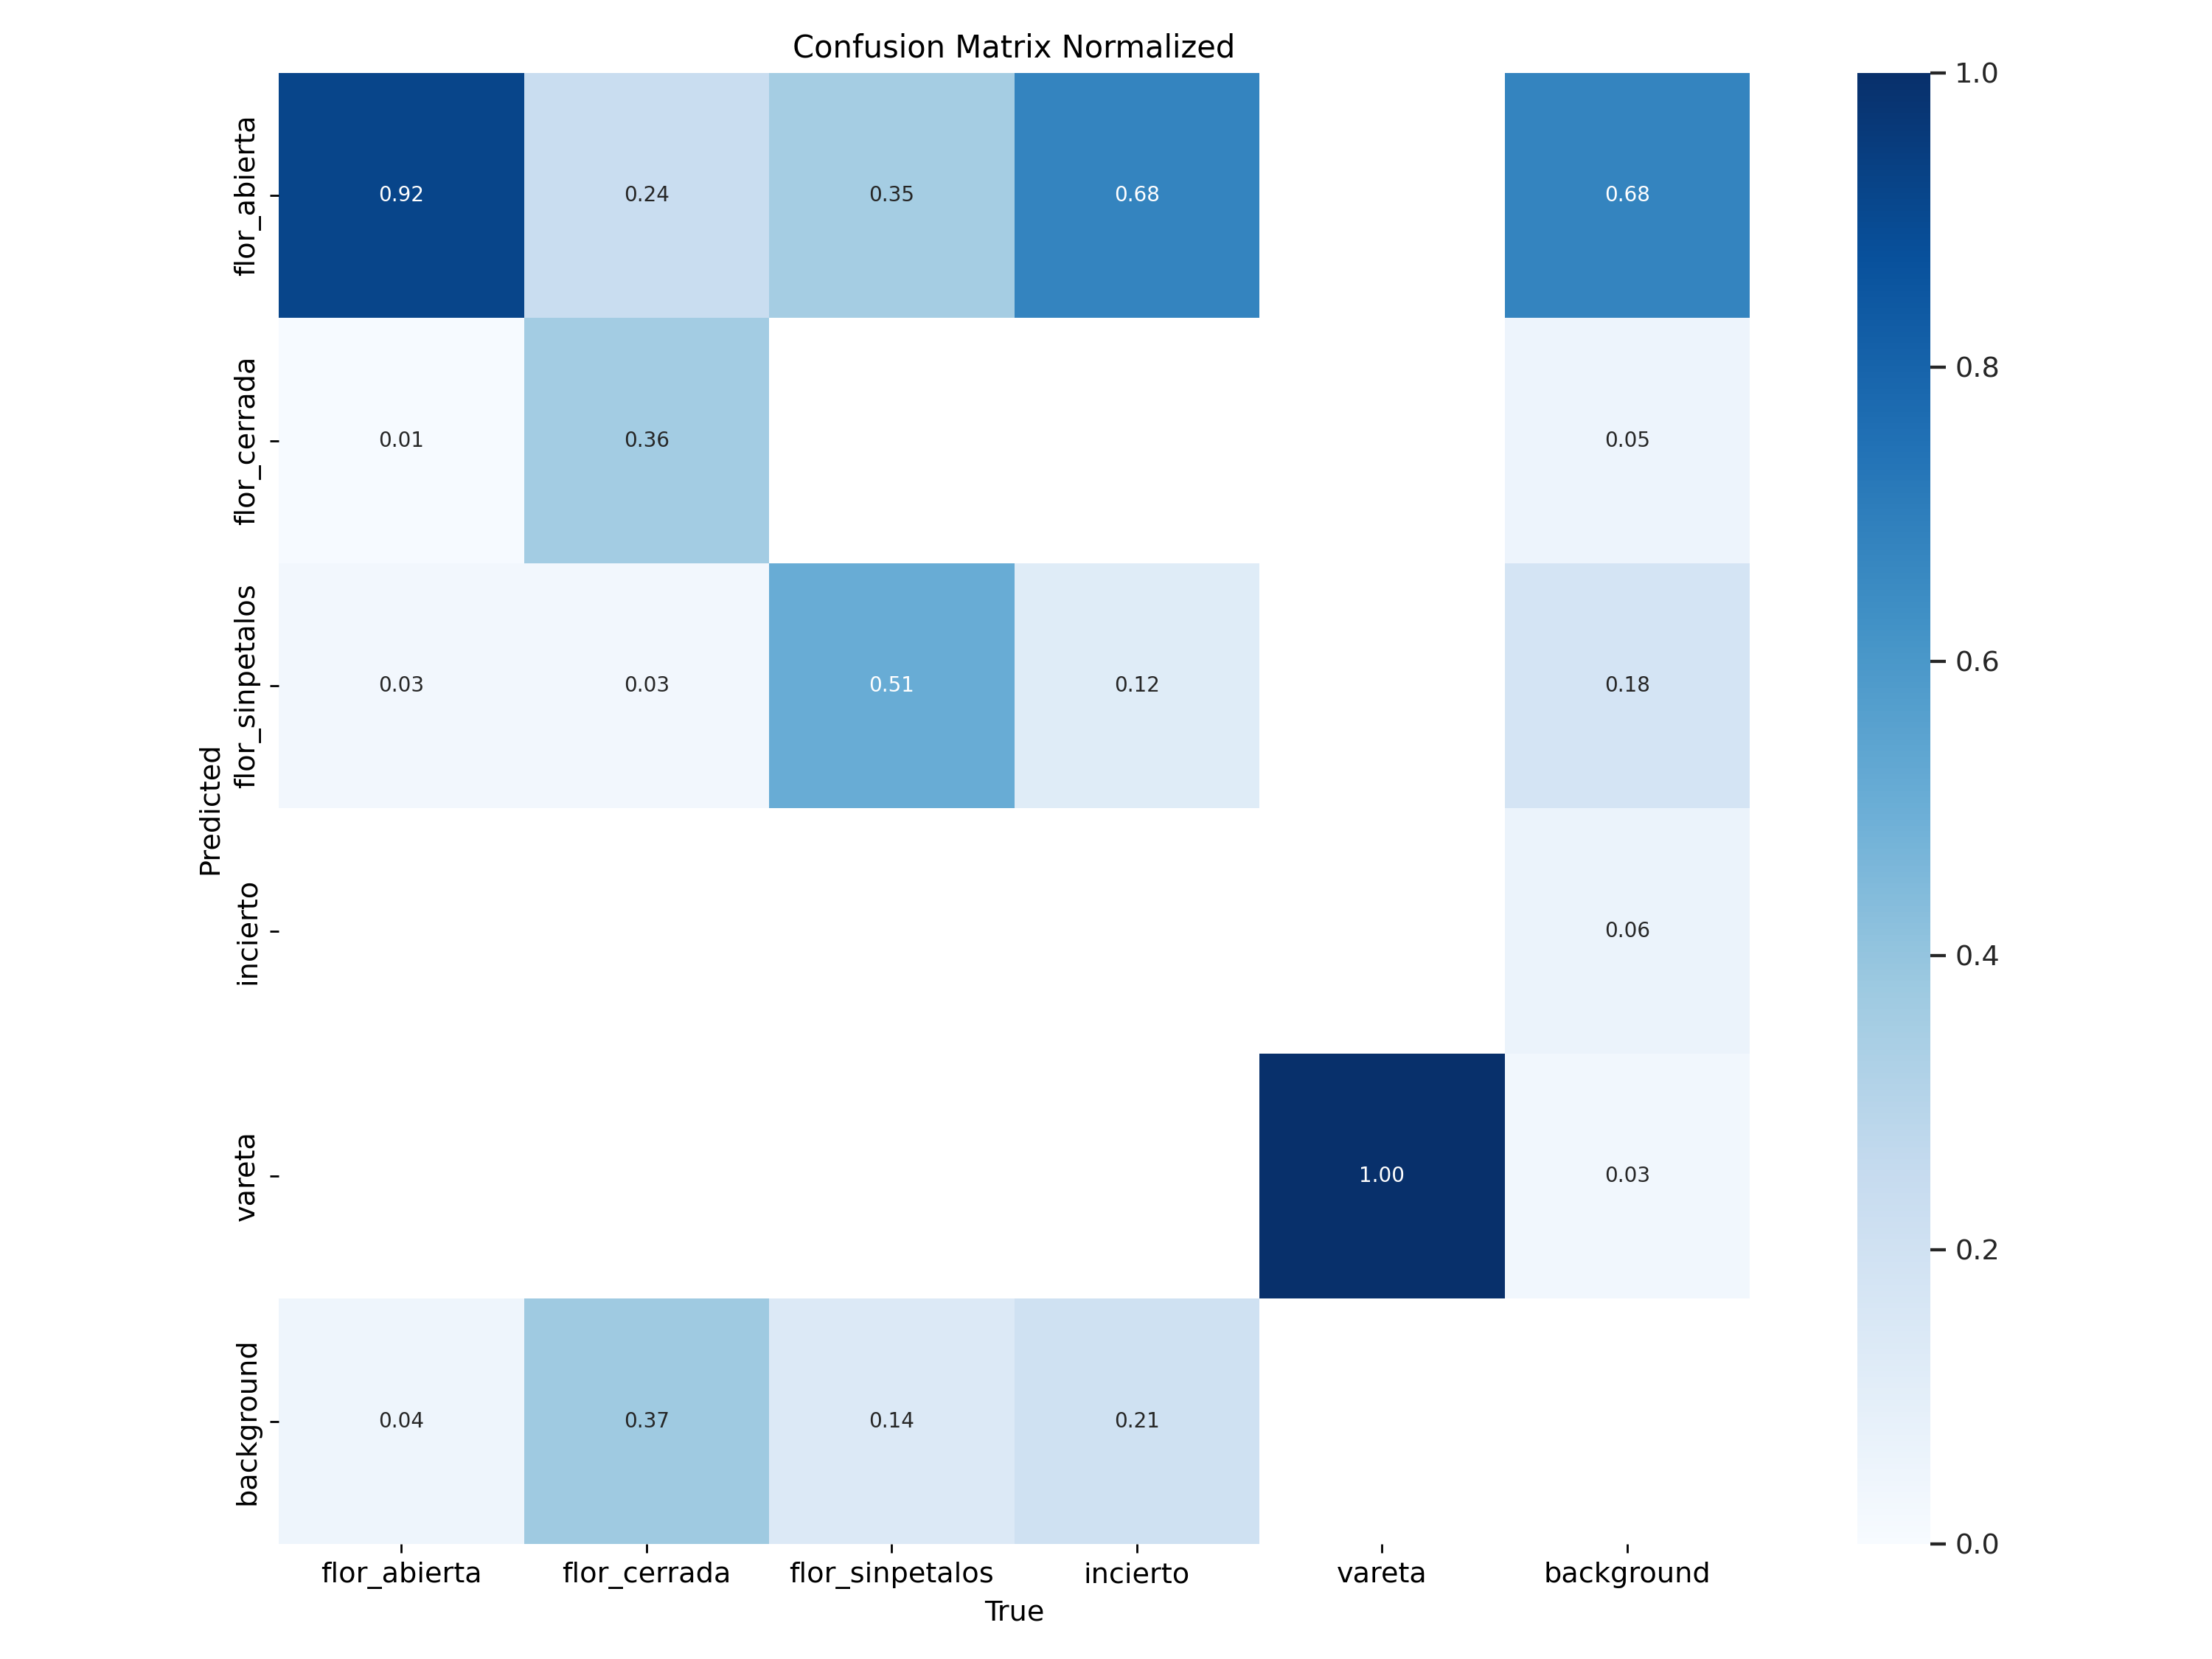
\includegraphics[scale=0.49]{./Figures/CFMatrixnorm.png}
	\caption{Matriz de confusión normalizada de YOLOv8n para el conjunto de prueba.}
	\label{fig:cfmatriznorm}
\end{figure}
\newpage
\subsubsection{YOLOv8n con aumento de datos}
\label{YOLOv8n con aumento de dato}

Para mejorar los resultados de YOLOv8n se implementó el aumento de datos descrito en la sección \ref{aumentoDatos}. Los resultados obtenidos contra el conjunto de imágenes de prueba, se observa en la tabla \ref{tab:resultadosYoloConAug}.

\begin{table}[h]
	\centering
	\caption{Métricas de detección para YOLOv8n con aumento de datos.}
	\begin{tabular}{c c c c c c c}    
		\toprule
		\textbf{Clase}&\textbf{Imágenes}&\textbf{mAP50}&\textbf{mAP>50}\\
		\midrule
		Todas & 14 & 0,655 & 0,423\\
		Flor abierta & 14 & 0,893 & 0,611 \\
		Flor cerrada & 14 & 0,673 & 0,266 \\
		Flor sin pétalos & 14 & 0,603 & 0,373 \\
		Incierto & 14 & 0,111 & 0,065 \\
		Vareta & 14 & 0,995 & 0,802 \\		
		\bottomrule
		\hline
	\end{tabular}
	\label{tab:resultadosYoloConAug}
\end{table}

La precisión promedio para un umbral de confianza igual al 50\% mejora para la clase flor cerrada en un 5,9\% y para la clase flor sin pétalos en un 1,5\%. Por otro lado, para la clase flor abierta se observa una pérdida del 1,2\%. De esta forma, se observa un aumento del 1\% para el mAP 50 de todas las clases.

Se observa que el entrenamiento del modelo con aumento de datos ayudó a mejorar el reconocimiento de las clases más difíciles de detectar como son flor cerrada y flor sin pétalos. Además, mantiene el buen rendimiento para las clases flor abierta y vareta.

Al comparar todos los experimentos realizados para la detección de los estados fenológicos de las flores de duraznero, el modelo con mejor rendimiento basado en la métrica mAP para dicha tarea es YOLOv8n con aumento de datos. Por este motivo, se seleccionó este modelo para desempeñar dicha tarea. Adicionalmente, este modelo es capaz de mitigar el desbalance de clases por su mecanismo interno que hace uso del \textit{Focal Loss} \cite{ARTICLE:15} para asignar mayor peso a las clases menos frecuentes en forma automática. 

Por último, se aplicó Eigen-CAM \cite{ARTICLE:17} para crear mapas de calor que permitan explicar los resultados obtenidos por el modelo. Este mapa de calor se implementó en la capa convolucional \textit{C2f}. En la figura \ref{fig:EigenCam} se observa un ejemplo de los mapas de calor generados por Eigen-CAM en una foto perteneciente al conjunto de pruebas utilizando YOLOv8n con aumento de datos.

\begin{figure}[ht]
	\centering
	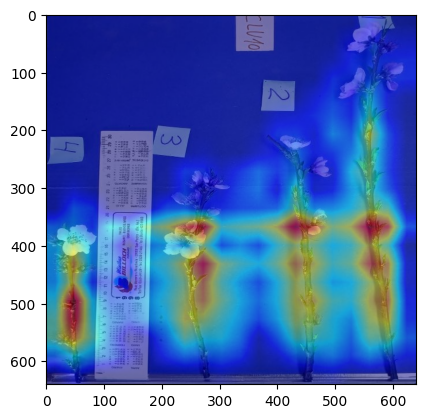
\includegraphics[scale=0.55]{./Figures/EigenCamEj.png}
	\caption{Mapa de calor con Eigen-CAM en la capa C2f del modelo YOLOv8n.}
	\label{fig:EigenCam}
\end{figure}

Se observa que los mapas de activación están enfocados en las varetas para la capa convolucional seleccionada, lo que sugiere que el modelo pone mayor atención en este objeto al momento de realizar la detección. 

\subsection{Desempeño del clasificador de flores}

El entrenamiento del clasificador de flores se realizó con los siguientes hiperparámentros.

\begin{itemize}
	\item Épocas: 50.
    \item Tamaño de imagen de entrada: 25 x 25.
    \item \textit{Batch}: 4.
    \item \textit{Learning rate}: 0,0001.
\end{itemize}


El clasificador de flores como se mencionó en el capítulo anterior, fue entrenado inicialmente sin ningún método de regulación, lo que terminó generando un sobreajuste a los datos de entrenamiento. En la figura \ref{fig:e1} se puede observar este sobreajuste.

\begin{figure}[ht]
	\centering
	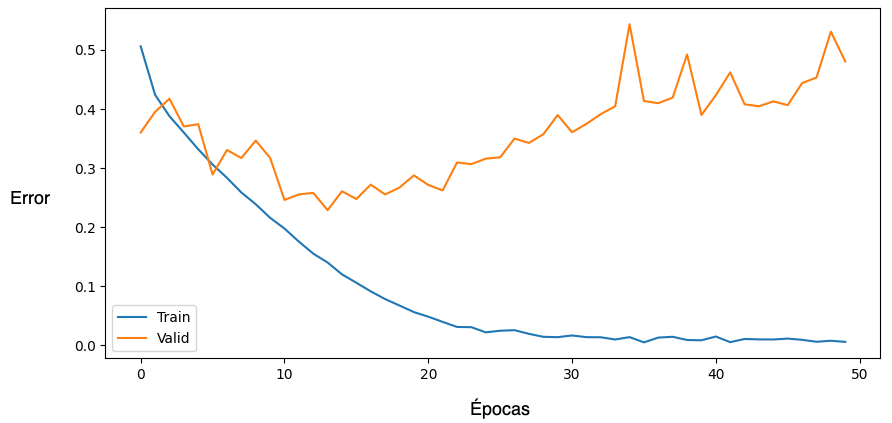
\includegraphics[scale=0.4]{./Figures/z.drawio.png}
	\caption{Error de entrenamiento vs validación sin métodos de regulación.}
	\label{fig:e1}
\end{figure}

Posteriormente se utilizó regulación L2 y \textit{DropOut} para disminuir el sobreajuste. Los valores aplicados en ambos casos fueron los siguientes.

\begin{itemize}
	\item L2: 0,01.
    \item \textit{DropOut}: 25\%.
\end{itemize}

En la figura \ref{fig:e2} se observa el resultado de aplicar ambos métodos de regulación.

\begin{figure}[ht]
	\centering
	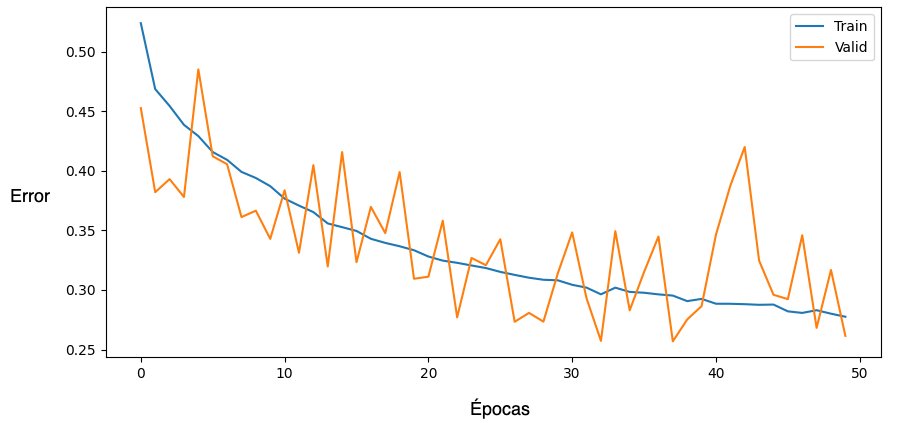
\includegraphics[scale=0.4]{./Figures/x.drawio.png}
	\caption{Error de entrenamiento vs validación con métodos de regulación.}
	\label{fig:e2}
\end{figure}

Por otro lado, para evaluar el desempeño del clasificador de flores se realizaron validaciones contra el conjunto de datos de prueba. Los resultados fueron medidos con las métricas \textit{accuracy}, \textit{precision}, \textit{recall} y F1. En la tabla \ref{tab:resultadosClass007} se muestran dichos resultados.

\begin{table}[h]
	\centering
	\caption{Métricas tomadas del clasificador de flores.}
	\begin{tabular}{c c c c c c c}    
		\toprule
		\textbf{\textit{Accuracy}}&\textbf{\textit{Precision}}&\textbf{\textit{Recall}}&\textbf{F1}\\
		\midrule
		0,87 & 0,82 & 0,81 & 0,87\\		
		\bottomrule
		\hline
	\end{tabular}
	\label{tab:resultadosClass007}
\end{table}
\newpage
De los resultados se puede concluir que el modelo logra clasificar con muy buena precisión ambas clases, a pesar del desbalance de datos observado en el capítulo anterior.

\section{Desempeño de módulos}
\label{sec:desempeñoModulos}

Como se mencionó en secciones anteriores, el sistema cuenta con dos módulos, y para estimar su desempeño se utiliza un método visual. Este método implica la introducción de una imagen o fotografía en el sistema, de manera que esta transite a través de cada módulo de manera secuencial. Posteriormente, se realiza una observación de la salida generada por cada módulo de forma individual y se toman conclusiones de su funcionamiento. Esta aproximación no solo facilita la medición del rendimiento del sistema en su totalidad, sino que también permite un examen detallado de las contribuciones y funcionalidades específicas de cada uno de sus componentes modulares.

\subsection{Desempeño del módulo de estimación de longitud}

El funcionamiento y precisión del módulo de estimación de longitud está relacionado a la calidad de las imágenes que recibe a la entrada. Estas imágenes tienen que contar con la regla de 30 centímetros como objeto de referencia y con condiciones similares a las que se presentaron en el entrenamiento del modelo (ejemplo: fondo, separación entre varetas, etc).

Por otro lado, en esta prueba de desempeño, se toma en cuenta la medición del objeto de interés y visualmente se compara la medición de la vareta más cercana a la regla, donde se podrá observar si su longitud visual es parecida a la estimada por el algoritmo. Además, se destaca que la medida se presenta en centímetros.

En la figura \ref{fig:DempeñoEstimacionLongitud}, se observa la prueba realizada para conocer el desempeño de este módulo.

\begin{figure}[ht]
	\centering
	\includegraphics[scale=0.35]{./Figures/DesempeñoMod1 (1).png}
	\caption{Desempeño del módulo de estimación de longitud.}
	\label{fig:DempeñoEstimacionLongitud}
\end{figure}
\newpage

Como se puede observar, la vareta con la etiqueta número cuatro mide 26,27 centímetros según el algoritmo. Sin embargo, visualmente aparenta medir 27 centímetros aproximadamente, lo que sugiere un error de medición de 0,73 centímetros. Adicionalmente, si se observa la vareta con la etiqueta número tres, su longitud según el algoritmo es de 29,60 centímetros, pero visualmente se aproxima a 30 centímetros, por lo que se presume un error de 0,4 centímetros. 

Con este resultado se puede concluir que el módulo aproxima la longitud de las varetas a valores muy cercanos a los que se obtienen visualmente. Sin embargo, al no poder medir con exactitud la longitud real de ambas varetas no se puede obtener con precisión el rendimiento de este módulo. Además, cabe destacar que esta medida se obtiene de forma lineal y no se cuentan las curvaturas de las varetas, lo que implica que esta medida no es exacta.

\subsection{Desempeño del módulo de detección y procesamiento}

Este módulo, como se mencionó en la sección anterior, realiza múltiples operaciones donde detecta los estados fenológicos, hace un conteo de la cantidad de flores en la imagen y por vareta, cuenta la cantidad de varetas y determina la cantidad de flores que se tienen en un estado o en otro.

En la figura \ref{fig:DesempeñoMod2}, se muestra una foto de varetas con los centroides pertenecientes a las detecciones realizadas. De este forma, es más simple evaluar y realizar el conteo de flores de forma visual, luego compararlo con los resultados obtenidos por el algoritmo que se detallan en la tabla \ref{tab:resultadosmod2}.

\begin{figure}[ht]
	\centering
	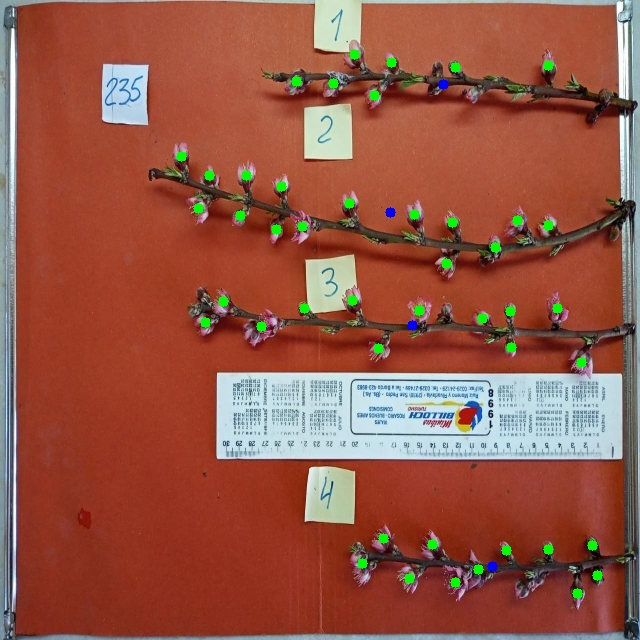
\includegraphics[scale=0.5]{./Figures/centroids3.jpeg}
	\caption{Desempeño del módulo de detección y procesamiento con el uso de centroides con flores campanuláceas.}
	\label{fig:DesempeñoMod2}
\end{figure}
\newpage

\begin{table}[h]
	\centering
	\caption{Tabla de resultados del módulo de detección y procesamiento para la imagen de muestra.}
	\begin{tabular}{c c c c c c c}    
		\toprule
		\textbf{Id}&\textbf{N° flores}&\textbf{Abiertas}&\textbf{Cerradas}&\textbf{Sin pétalos} &\textbf{Tipo}\\
		\midrule
		1 & 7 & 6 & 1 & 0 &  Campanulácea\\
		2 & 15 & 13 & 2 & 0 &  Campanulácea\\
		3 & 12 & 9 & 2 & 0 &  Campanulácea\\
		4 & 11 & 6 & 5 & 0 &  Campanulácea\\
		Total & 45 & - & - &  - & - \\
		N° varetas & 4 & - &  - & - & - \\
		\bottomrule
		\hline
	\end{tabular}
	\label{tab:resultadosmod2}
\end{table}


Se toma como muestra la vareta con el identificador número cuatro, donde el algoritmo indica que existen un total de once flores. Luego, al realizar el conteo visual, se encuentran un total de trece flores. De estas trece flores, las dos flores que no pudo detectar el algoritmo con sus valores por defecto (nivel de confianza igual a 0,4) son flores cerradas. Por otro lado, el algoritmo señala que de las once flores, hay seis abiertas y cinco cerradas. Visualmente se detectan seis flores abiertas (como menciona el algoritmo) y siete flores cerradas. Con esto, se puede concluir y corroborar que la detección y las tareas derivadas que ejecuta este módulo son impactadas por el rendimiento del modelo base detallado en la sección \ref{YOLOv8n con aumento de dato}, donde se observa que el modelo tiene una alta precisión para detectar las flores en estado abierto, pero la precisión es menor para las demás clases relacionadas a los otros estados fenológicos.

Además, de los resultados se destaca que para cada vareta el tipo de flor encontrada por el clasificador fue del tipo campanulácea, lo que coincide con lo observable en la imagen de muestra. Igualmente se remarca el buen funcionamiento del módulo en la detección de las cuatro varetas encontradas en la imagen.